\documentclass[crop,tikz]{standalone}
\usepackage{xcolor,amsmath,booktabs}
\usetikzlibrary{arrows,automata,decorations.pathreplacing,patterns}

\setlength{\textwidth}{513pt}

% color palette
\colorlet{anthracite}{black!90}
\definecolor{tu01}{HTML}{84B818}
\definecolor{tu03}{HTML}{1BB5B5}
\definecolor{tu06}{HTML}{E3B505}

% mixed and light colors
\colorlet{tu01light}{tu01!36}
\colorlet{tu03light}{tu03!32}
\colorlet{tu06light}{tu06!28}

% layer styles
\tikzstyle{dense layer} = [%
	state,
	rectangle,
	draw=anthracite,
	minimum height=14mm,
	rounded corners=2pt,
	pattern = north east lines,
	pattern color = black!10
]
\tikzstyle{dense layer a} = [%
	dense layer,
	minimum width=5mm,
	% pattern = north east lines,
	% pattern color=tu01light
]
\tikzstyle{dense layer b} = [%
	dense layer,
	minimum width=3mm,
	% pattern = crosshatch dots,
	% pattern color=tu03light
]
\tikzstyle{dense layer c} = [%
	dense layer,
	minimum width=2mm,
	minimum height=10mm,
	% pattern = crosshatch,
	% pattern color=tu06light
]

% edges
\tikzset{every edge/.append style={
	->,
	>=stealth',
	shorten >=2pt,
	auto,
	semithick
}}

% labels and braces
\tikzstyle{input} = [%
	state,
	rectangle,
	draw=none,
	align=center,
	inner sep=4pt,
	anchor=west,
	font=\footnotesize
]
\tikzstyle{underbrace} = [thick, decoration={brace, mirror, raise=1mm}, decorate]
\tikzstyle{underbrace label} = [midway, anchor=north, yshift=3mm, text width=60mm, align=center, font=\scriptsize\ttfamily]
\tikzstyle{overbrace} = [thick, decoration={brace, raise=1mm}, decorate]
\tikzstyle{overbrace label} = [midway, anchor=south, yshift=1.5mm, text width=60mm, align=center, font=\scriptsize\ttfamily]

\begin{document}
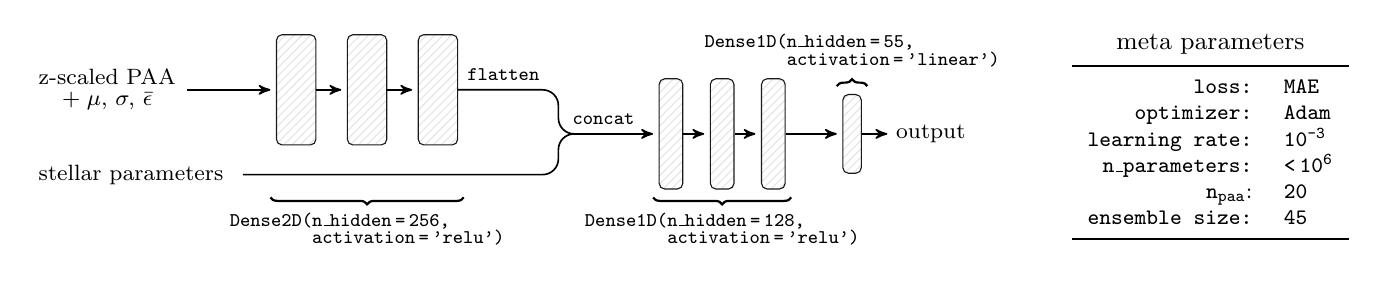
\begin{tikzpicture}[x=\textwidth]

% \draw[gray] (0,1cm) -- (1,1cm);


% first network part with input
\node[input] (paa) at (0,0) {%
	z-scaled PAA\\[-2pt]$+ \; \mu, \, \sigma, \, \bar{\epsilon}$
};
\begin{scope}[node distance=9mm]
	\node[dense layer a, right of=paa, xshift=15mm] (a1) {};
	\node[dense layer a, right of=a1] (a2) {};
	\node[dense layer a, right of=a2] (a3) {};
	\path (paa) edge (a1)
	      (a1) edge (a2)
	      (a2) edge (a3);
\end{scope}

% second network part with final layer
\begin{scope}[node distance=6.5mm]
	\node[dense layer b, below right of=a3, shift={(25mm, -1mm)}] (b1) {};
	\node[dense layer b, right of=b1] (b2) {};
	\node[dense layer b, right of=b2] (b3) {};
	\node[dense layer c, right of=b3, xshift=3.5mm] (c1) {};
	\node[input, right of=c1, minimum width=0mm, inner sep=1pt, xshift=3.5mm] (output) {output};
	\path (b1) edge (b2)
	      (b2) edge (b3)
	      (b3) edge (c1)
	      (c1) edge (output);
\end{scope}

% braces
\draw [underbrace] ([xshift=-2pt] a1.south west|-b1.south west) -- ([xshift=2pt] a3.south east|-b3.south east)
 node [underbrace label] {%
	\begin{align*}
		\text{Dense2D(}&\text{n\_hidden\,=\,256,}\\[-1.6mm]&\text{activation\,=\,'relu')}
	\end{align*}
}; % first part
\draw [underbrace] ([xshift=-2pt] b1.south west) -- ([xshift=2pt] b3.south east)
 node [underbrace label] {%
	\begin{align*}
		\text{Dense1D(}&\text{n\_hidden\,=\,128,}\\[-1.6mm]&\text{activation\,=\,'relu')}
	\end{align*}
}; % second part
\draw [overbrace] ([xshift=-2pt] c1.north west) -- ([xshift=2pt] c1.north east)
 node [overbrace label] {%
    ~\vspace{-5mm}
	\begin{align*}
		\text{Dense1D(}&\text{n\_hidden\,=\,55,}\\[-1.6mm]&\text{activation\,=\,'linear')}
	\end{align*}
}; % final layer

% auxiliary input and concatenation
\path (a1.south) -- ([yshift=-1.8mm]b1.south) coordinate[midway] (stellar y);
\node[input, align=left] (stellar) at (paa.west|-stellar y) {%
	stellar parameters
};
\path (a3.east) -- (b1.west) coordinate[midway] (joint x);
\coordinate (joint) at (joint x|-b1);
\draw[semithick, rounded corners=2mm]
  (stellar) -- (joint|-stellar) -- (joint) -- ([xshift=2mm] joint)
  (a3.east) -- (joint|-a3.east) -- (joint) -- ([xshift=2mm] joint);
\path ([xshift=2mm] joint) edge (b1);
\path (a3.east) -- node[pos=.45, above, font=\ttfamily\scriptsize] {flatten} (joint|-a3.west);
\path (joint) -- node[pos=.45, above, font=\ttfamily\scriptsize] {concat} (b1);

% parameter table
\path (current bounding box.north) -- (current bounding box.south) coordinate[midway] (box mid);
\coordinate (page east) at (\textwidth,0);
\node[%
	state,
	rectangle,
	anchor=north east,
	font=\footnotesize,
	draw=none,
	inner sep=1pt
] at ([xshift=-12mm] page east|-current bounding box.north) {%
	\setlength{\tabcolsep}{2mm}
	\begin{tabular}{rl}
		\multicolumn{2}{c}{\small meta parameters} \\[1mm]
		\toprule
		\texttt{loss:} & \texttt{MAE} \\
		\texttt{optimizer:} & \texttt{Adam} \\
		\texttt{learning rate:} & $\text{\texttt{10}}^\text{\texttt{-3}}$ \\
		\texttt{n\_parameters:} & $\text{\texttt{<\,10}}^\text{\texttt{6}}$ \\
		$\text{\texttt{n}}_\text{\texttt{paa}}$: & \texttt{20} \\
		\texttt{ensemble size:} & \texttt{45} \\
		\bottomrule
	\end{tabular}
};

% 10^6 parameters

\end{tikzpicture}
\end{document}
